Innanzitutto sono stati analizzati i ``Determinanti'', cioè le attività umane (determinanti antropici) e il contesto meteo-climatico (determinanti naturali) rilevanti ai fini della qualità dell'aria. L'analisi dei determinanti antropici deve fare i conti con la limitatezza di informazioni disponibili in tempi brevi. Molti degli indicatori usualmente considerati nella redazione degli inventari delle emissioni in atmosfera sono disponibili solo su base annua, spesso solamente alcuni mesi dopo la fine dell'anno. Pertanto in questo report si sono potuti considerare indicatori relativi al traffico su strada e al traffico aeroportuale, accessibili tempestivamente grazie alla collaborazione di alcuni Enti ed Aziende (Tab.\ref{tab:datasources}).

Mancano informazioni sulla variazione nei consumi per il riscaldamento domestico e sulle attività industriali, mentre per agricoltura e allevamento si può ipotizzare che le attività rilevanti ai fini della qualità dell'aria non abbiano registrato variazioni attribuibili alle azioni di contenimento di COVID-19.


\subsection{Traffico su strada}

Sono state raccolte informazioni sugli andamenti settimanali del traffico sulle varie tipologie di strade, ove disponibili disaggregate per tipologia di veicoli (fig.\ref{fig:riduzionedeterminanti}).
\paragraph{Strade urbane}
Per stimare l'andamento settimanale del traffico veicolare sulle strade urbane, sono state considerate (tab.\ref{tab:datasources}) per il periodo 22/2--13/3/2020 le statistiche elaborate da Fondazione ISI su dati Cuebiq \citep{pepe2020covid}\footnote{disponibili all'indirizzo https://data.humdata.org/dataset/covid-19-mobility-italy}, in particolare il \textit{radius of gyration} mediano settimanale delle quattro province del FVG. Per le settimane seguenti si sono considerati i conteggi di veicoli, forniti dal Comune di Pordenone su base mensile, ipotizzando un calo lineare nel corso delle settimane fino alla fine di marzo. Non disponendo di informazioni differenziate per tipologia di veicolo, l'andamento è stato considerato valido per tutte le tipologie.

I volumi di traffico urbani si sono ridotti dalla quarta settimana di febbraio fino a registrare un calo del 76\% a fine marzo (fig.\ref{fig:riduzionedeterminanti}, primo pannello).

\paragraph{Strade extra-urbane}
Per stimare l'andamento settimanale del traffico veicolare sulle strade extra-urbane, sono stati considerati (tab.\ref{tab:datasources}) per il periodo 1/2--31/3 i volumi di traffico, stratificati per tipologia di veicolo, riferiti a 10 postazioni collocate lungo strade dell'Isontino e della pianura friulana orientale. L'andamento del 2020 è stato confrontato giorno per giorno con l'andamento mediano dei due anni precedenti, calcolato sul medesimo giorno della settimana e sul medesimo mese. 

I volumi di traffico su strade extra-urbane si sono ridotti dalla quarta settimana di febbraio fino a raggiungere a fine marzo riduzioni comprese tra il -87\% degli autoveicoli e il -68\% dei veicoli commerciali pesanti (fig.\ref{fig:riduzionedeterminanti}, secondo pannello).

\paragraph{Autostrade}
Per stimare l'andamento settimanale del traffico veicolare sulle autostrade, sono stati considerati (tab.\ref{tab:datasources}) per il periodo 1/1--31/3 le percorrenze totali registrate da Autovie Venete nelle tratte autostradali di propria competenza, stratificate per tipologia di veicolo. L'andamento del 2020 è stato confrontato giorno per giorno con l'andamento dell'anno precedente, spostandolo di una giornata per far coincidere il giorno della settimana.

Le percorrenze totali sulle autostrade (fig.\ref{fig:riduzionedeterminanti}, terzo pannello) si sono notevolmente ridotte per i veicoli leggeri (fino a -91\%), meno sensibilmente per i veicoli pesanti (-53\% a fine marzo).

\subsection{Traffico aereo}
Il numero di voli quotidiani forniti da Trieste Airport (tab.\ref{tab:datasources}) è stato confrontato su base settimanale con la media dei numeri di voli nelle medesime settimane degli anni 2011--2013 e 2015. Inoltre, sono state considerate le variazioni dei consumi di gasolio dei mezzi aeroportuali a terra nei mesi di febbraio e marzo, rispetto a gennaio 2020; gli andamenti mensili dei consumi sono stati disaggregati su base settimanale ipotizzando una dipendenza lineare dal numero di voli.

Il traffico aereo è stato drasticamente ridotto (fig.\ref{fig:riduzionedeterminanti}, ultimo pannello), fino ad azzerarsi nelle ultime settimane di marzo.

\begin{landscape}
\begin{table}[ht]
    \caption{Informazioni e dati raccolti da ARPA-FVG relativi ai determinanti, per il periodo analizzato}
    \centering
 \begin{tabular}{p{0.19\textwidth}p{0.22\textwidth}lp{0.4\textwidth}p{0.28\textwidth}}
    \toprule
        settore & \multicolumn{2}{c}{copertura} & descrizione & fonte \\
        \cmidrule{2-3}
        &spaziale & temporale &&\\
        \midrule
        trasporto su strada & FVG & 1/1--31/3 & volumi di traffico su autostrade & Autovie Venete \\
         & pianura friulana orientale e Isontino & 1/2--31/3 & flussi di traffico su strade extra-urbane & RAFVG (Infrastrutture e Territorio)\\
         & Pordenone & 1/2--22/4 & flussi di traffico su strade urbane & Comune di Pordenone\\
         & FVG & 22/2--13/3 & indici di mobilità & Cuebiq, Fondazione ISI\\
         & Italia, FVG & 1/2--14/4 & volumi di traffico giornalieri & ANAS\\
%         & FVG & & carburante venduto per autotrazione & \\
        trasporto aereo & scala mondiale & & numero di voli tracciati & flightradar.com\\
         & Aeroporto di Trieste & 1/1--2/4 & numero di voli giornalieri & Trieste Airport\\
         &                      & 1/1--31/3& consumi di carburante dei mezzi aeroportuali & Trieste Airport\\
 %       trasporto ferroviario & FVG & & \\
 %       riscaldamento domestico & FVG & & \\
        agricoltura & FVG & 1/11--22/3 & calendario delle autorizzazioni agli spandimenti di liquami zootecnici & RAFVG (Risorse Agroalimentari. Forestali e Ittiche)\\
        \bottomrule
    \end{tabular}
    \label{tab:datasources}
\end{table}
\end{landscape}

\begin{figure}
    \centering
    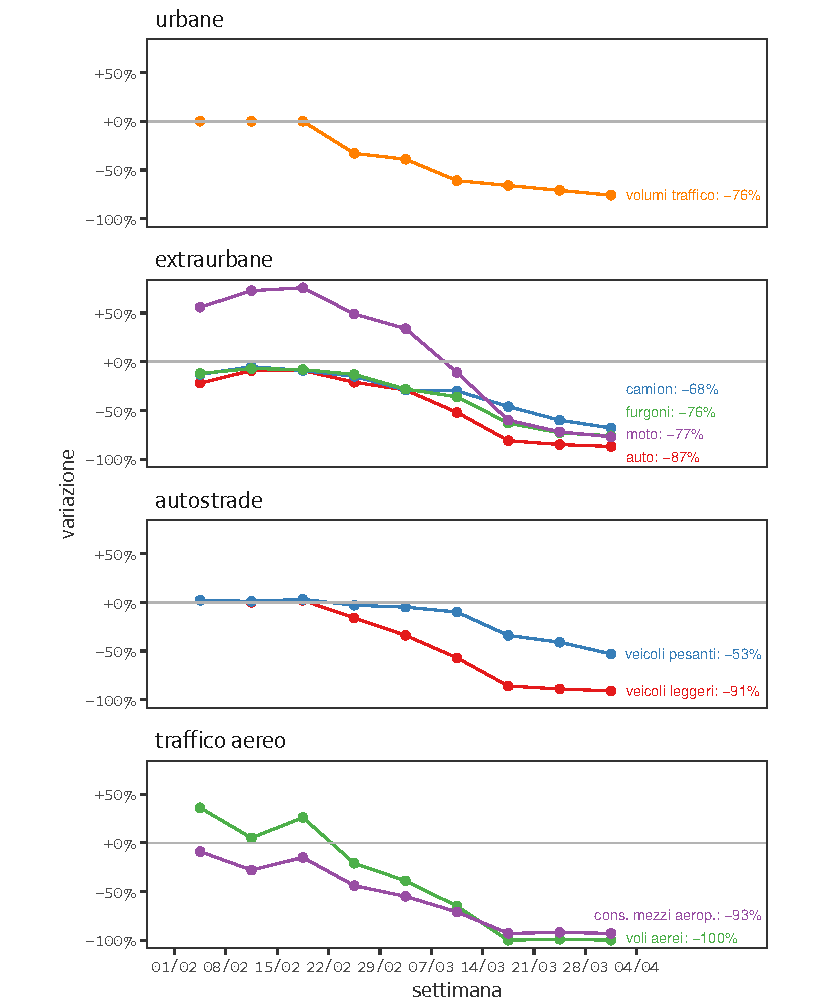
\includegraphics[width=\textwidth]{{figs/riduzioniDeterminanti_20200201-20200331}.pdf}
    \caption[Variazioni di indicatori relativi ad attività antropiche]{Variazioni settimanali di alcuni indicatori relativi ad attività antropiche rilevanti per la qualità dell'aria. Dall'alto: traffico su strade urbane, extra-urbane e autostrade; in fondo: traffico aereo.}
    \label{fig:riduzionedeterminanti}
\end{figure}
